%%%%%%%%%%%%%%%%%%%%%%%%%%%%%%%%%%%%%%%%%%%%%%%%%%%%%%%%%%%%%%%%%%%%%%%%%%%%%%%%
%2345678901234567890123456789012345678901234567890123456789012345678901234567890
%        1         2         3         4         5         6         7         8

\documentclass[letterpaper, 10 pt, conference]{ieeeconf} % Comment this line out if you need a4paper

%\documentclass[a4paper, 10pt, conference]{ieeeconf}      % Use this line for a4 paper

\IEEEoverridecommandlockouts                              % This command is only needed if 
                                                          % you want to use the \thanks command

\overrideIEEEmargins                                      % Needed to meet printer requirements.

%In case you encounter the following error:
%Error 1010 The PDF file may be corrupt (unable to open PDF file) OR
%Error 1000 An error occurred while parsing a contents stream. Unable to analyze the PDF file.
%This is a known problem with pdfLaTeX conversion filter. The file cannot be opened with acrobat reader
%Please use one of the alternatives below to circumvent this error by uncommenting one or the other
%\pdfobjcompresslevel=0
%\pdfminorversion=4

% See the \addtolength command later in the file to balance the column lengths
% on the last page of the document

% The following packages can be found on http:\\www.ctan.org
%\usepackage{graphics} % for pdf, bitmapped graphics files
%\usepackage{epsfig} % for postscript graphics files
%\usepackage{mathptmx} % assumes new font selection scheme installed
%\usepackage{times} % assumes new font selection scheme installed
%\usepackage{amsmath} % assumes amsmath package installed
%\usepackage{amssymb}  % assumes amsmath package installed

\usepackage{circledsteps}
\usepackage{newtxtext,newtxmath}
\usepackage{xspace}
\usepackage{caption}
\usepackage{subcaption}
\usepackage{todonotes}
\usepackage{float}
\usepackage{cite}
\usepackage{hyperref}
\usepackage{multirow}
\usepackage{booktabs}

\newcommand{\neuroflight}{NeuroFlight\xspace}
\newcommand{\tf}{Tensor Flow\xspace}
\newcommand{\tflite}{\textit{TF-lite}\xspace}
\newcommand{\gstation}{Ground Station\xspace}
\newcommand{\drone}{Drone\xspace}
\newcommand{\xbee}{RF\xspace}
\newcommand{\gyro}{Gyroscope\xspace}
\newcommand{\obs}{Observation\xspace}
\newcommand{\note}[1]{\textcolor{red}{#1}}
\newcommand{\pDDPGx}{$\psi\text{DDPG}\times$}
\newcommand{\DDPGx}{$\text{DDPG}\times$}

\newcommand{\firmwarelong}{Swappable Neural Network Flight control}
\newcommand{\firmware}{SwaNNFlight}
\newcommand{\framework}{SwaNNS}
\newcommand{\frameworklong}{SwaNN Station}
\newcommand{\rev}[1]{\textcolor{black}{#1}}


\title{\LARGE \bf
Anchored Learning for On-the-Fly Adaptation
}

\author{Bassel El Mabsout$^{1}$, Siddharth Mysore$^{1}$, Shahin Roozkhosh$^{1}$, Kate Saenko$^{1,2}$ and Renato Mancuso$^{1}$% <-this % stops a space
% \thanks{*This work was not supported by any organization}% <-this % stops a space
\thanks{$^{1}$Affiliated with the Computer Science department at Boston University}%
\thanks{$^{2}$Co-affiliated with the MIT-IBM Watson AI Lab}%
}
% \author{Albert Author$^{1}$ and Bernard D. Researcher$^{2}$% <-this % stops a space
% \thanks{*This work was not supported by any organization}% <-this % stops a space
% \thanks{$^{1}$Albert Author is with Faculty of Electrical Engineering, Mathematics and Computer Science,
%         University of Twente, 7500 AE Enschede, The Netherlands
%         {\tt\small albert.author@papercept.net}}%
% \thanks{$^{2}$Bernard D. Researcheris with the Department of Electrical Engineering, Wright State University,
%         Dayton, OH 45435, USA
%         {\tt\small b.d.researcher@ieee.org}}%
% }


\begin{document}



\maketitle
\thispagestyle{empty}
\pagestyle{empty}


% [fact] we want safe agents
% [fact] RL agents are often trained in sim
% [fact] There is sim-to-real gap
% [fact] sim-to-real ---> failure:
% [fact] failure can happen on multiple ground: eg. predictability + efficiency (power)
% [fact] to overcome sim-to-real gap --> community RL adaptation  ******
% [fact] for RL-adaptation to work, ---- certain distribution NICE *********

% [challenge] our focus: real-wrold scenarios, where distributions are not NICE. *********
% [vision] our focus: overcome catastrophic forgetting in RL *********
% [solution] our solutions: Anchors for having both safety while also 50percent efficient
% [contribution] we also -------- open-source shit

% Reinforcement Learning (RL) agents are typically honed in simulated settings, but they often encounter challenges such as unpredictability, excessive power consumption, and control failures when introduced to the real world, largely due to the disparity known as the "sim-to-real gap." Reducing this gap involves incorporating real-world data into the RL agents' training process. In simulations, agents can be tested on critical scenarios regardless of occurrence frequency, which is not the case with real-world data, leading to a skewed distribution that's harder to manage. Consequently, policies that maximize rewards based on common observations might result in unforeseen behaviors during infrequent but critical real-world situations, a phenomenon known as catastrophic forgetting.

% To address these issues, we propose a new approach called "anchor critics," which encourages RL agents to sustain their performance levels across both simulated and real-world environments, thereby preventing catastrophic forgetting. Our findings show that this methodology effectively improves the performance of RL agents, as demonstrated in both simulated environments and with actual racing quadrotors. Notably, it achieves nearly a 50% reduction in power consumption while also averting loss of control incidents.

% Furthermore, we are contributing \firmware{}, a versatile open-source firmware that facilitates the application of adaptation techniques on tangible robotic systems.

% Reinforcement learning (RL) agents are typically trained to perform well on critical scenarios in simulated environments but may struggle with unpredictability, excessive power use, and control failures when operating in the real world.
% These issues arise primarily due to the gap between simulation and reality.
% Narrowing this gap is feasible through the incorporation of real-world observations into the training of RL agents.
% However, the distribution of real-word observations is challenging to control.
% In combination with catastrophic forgetting of behaviors learnt in simulation, agents become unpredictable during rare real-world events.

% To address this, our research introduces 'anchor critics', a novel approach designed to improve agent robustness accross multiple domains, sustaining performance across both simulated and actual environments. Our findings indicate that anchor critics avert the issues caused by catastrohpic forgetting when subjected to multiple domains. This unlocked the ability to perform live-adaptation on real racing quadrotors producing a near 50\% reduction in power consumption. Additionally, we provide \firmware{}, our open-source firmware that facilitates the application of adaptation techniques on physical robots.




\begin{abstract}
This study presents ``anchor critics", a novel strategy developed to enhance the robustness of reinforcement learning (RL) agents in crossing the sim-to-real gap.
RL agents successfully trained in simulation often encounter difficulties such as unpredictability, inefficient power consumption, and operational failures when deployed in the real world.
A naive approach to bridging the sim-to-real gap involves fine-tuning agents on real-world data.
However, we observe that agents fine-tuned on real-world data achieve higher rewards on high-modality states, but suffer from catastrophic forgetting on states with low probability of occurence.
This results in unpredictable and unsafe behavior as the agents forget how to perform critical maneuvers that it had learned in simulation.
Since robots in the real world are often restricted to safe operation, such as in the case of quadrotors, this highlights the need for handling the shift in data distribution.
% Say something about how fine-tuning with real data can help but can also lead to catastrophic forgetting of lower-probability states
% Incorporating real-world data into the training pipeline can bridge the sim-to-real gap, but the distribution of real-world observations can be impossible to control.
Our findings indicate that the distributional shift of data from simulation and reality exacerbates catastrophic forgetting, causing well-behaved policies to rapidly lose control of the physical system on real-world low-probability states.
    % Reinforcement Learning (RL) agents are often trained to perform well in simulated environments.
    % Once deployed in the real world they can suffer from general unpredictability, high power consumption, and failure of control, mainly due to the sim-to-real gap.
    % This gap can be minimized by training RL agents with real-world observations.
    % However, unlike in simulation where we may evaluate agents over critical scenarios independent of their rate of occurrence. The distribution of real observations on the other hand may be difficult to control.
    % Catastrophic forgetting allows policies maximizing rewards on those observations to form unpredictable behaviors on rare real-world events.
    % Unlike in simulation where we can evaluate agents on critical scenarios, 
    % We present anchor critics, a mechanism incentivizing agents to maintain performance both in simulation and in reality, preventing catastrophic forgetting.
    We demonstrate that anchors both in simulated scenarios and on real racing quadrotors prevents loss of control, unlocking a near-50\% reduction in power consumption.
    We also contribute \firmware{}, an open-source firmware enabling testing adaptation techniques on real robots.
    % Via over-the-air updates of onboard control policies from a ground station.
    % Unnlocking a 
    % We also show that anchors prevent issues of catastrophic forgetting and controller instability both in simulation and in reality.
    Project Website: \url{https://github.com/BU-Cyber-Physical-Systems-Lab/SwaNNFS}
    % Achieving on-the-fly adaptation required the contribution of \firmware{}, an open-source firmware enabling wireless data capture and swapping of onboard Neural Network-based controllers \emph{live} with trivial overhead.
    % (i) The \frameworklong{} (\framework{}), an open source framework for training and live-adapt agents on similar systems. \framework{} contains \firmware{}, an open-source firmware enabling wireless data capture and swapping onboard NN controllers live with trivial overhead.
    % (i)  Allowing for 
    
    % (i) The open-source \framework{} (\framework{}), allows training and real-time adaptation of controllers while minimizing 
    % And (ii) Multiplicative value composition, a technique for preserving the importance of policy optimization criteria, improving training performance and variability in learned behaviors.
    
\end{abstract}


%%%%%%%%%%%%%%%%%%%%%%%%%%%%%%%%%%%%%%%%%%%%%%%%%%%%%%%%%%%%%%%%%%%%%%%%%%%%%%%%
\section{INTRODUCTION}

    Reinforcement Learning (RL) enables training policies to solve complex control problems for which traditional techniques may be ill-equipped.
    RL agents are often trained and evaluated in simulated environments due to the expensive nature of real-world robot interaction.
    % and while this is a good fit for applications such as video games, real-world robotic tasks require controllers (learned or otherwise) to be safe, reliable, and efficient. 
    % These properties are difficult to attain in learned controllers.
    Recent work has shown that these controllers applied to real systems can exhibit undesirable properties ranging from minor jerkiness, to over-heating due to the high power consumption of inefficient control policies, and even to hardware failures~\cite{benchmarkingRobo, Sim2Real, Sim2multi, benchmarkingRL, NFThesis}.
    These problems can be attributed to a failure of control policies to cross the domain gap between simulated training environments and the real world, i.e. the \emph{reality gap}.
    Despite this, simulated training remains attractive, as direct on-robot training raises important safety and expense concerns.
    Therefore, many existing works opt to train controllers in simulation, adapting them to reality via online optimization.

    \textit{(i) Anchors:}
    However, when attempting to naively adapt agents across multiple domains via traditional RL methods, we observed problems such as low performance, catastrophic forgetting, and complete loss of control.
    We attribute these issues to the shift in the distribution of data captured on-robot in contrast to the distribution chosen in simulation.  
    
    \noindent\textbf{Contribution:} We introduce \emph{anchor critics} for live adaptation, where the value function learned in simulation is preserved and used in tandem with a value function learned from data gathered on-robot.
    This approach demonstrably improves behavior retention while allowing policies to arbitrarily adapt to new environments, providing a novel solution to the problem of environmental distributional shifts. We demonstrate anchors on a suite of Gymnasium environments and observe a 50\% reduction in power draw on a real racing quadrotor.

    \textit{(ii) \firmware{}:}
    Robots are often built to minimize size, weight, power, and cost (SWaPc).
    This constrains the computational power available in the form of on-board embedded micro-controllers.
    Some methods circumvent this problem by offloading computations to a ground-station server for both training and inference of controllers.
    This inherently limits the robots' practicality, rendering them unusable upon communication failure.
    Often deployed in uncontrollable environments or requiring real-time control responses, robots such as self driving cars, rescue quadripeds, or racing quadrotors require the ability to perform inference on-board.
    
    In this work, we tackle live-adapting RL agents such that inference is performed on-board, while training is done on a ground station.
    As training can be much more expensive than optimized NN inference, we allow for sparse communication to tranceive policies and observations.
    
    \noindent\textbf{Contribution:} We introduce \firmwarelong{}~(\firmware{}), an open-source firmware which redesigns and extends Neuroflight~\cite{NFori,NFv2}.
    We built \firmware{} to support primitives for the transmission of observation data and for receiving and hot-swapping NN controllers during robot operation.
    And \frameworklong{}~(\framework{}) to enable receiving, training NN controllers with data acquired live, and transmitting updated policies.
    
    \framework{} and \firmware{} take care of training, deploying, and swapping neural-network (NN) models during live operation, allowing the research community to focus on experimenting with live-adaptation algorithms with support for many existing robotic platforms.
    
    \textit{(iii) Mulitplicative goal composition:} We observed a high variance in the quality of policies learned in simulation using actor-critic methods on a quadrotor control environment.
    
    \noindent\textbf{Contribution:} We thus opted to mulitplicatively compose policy optimization criteria, instead of linearly, substantially improving learning performance and variance.
    



%%%%%%%%%%%%%%%%%%%%%%%%%%%%%%%%%%%%%%%%%%%%%%%%%%%%%%%%%%%%%%%%%%%%%%%%%%%%%%%%
\section{\frameworklong{} FOR LIVE NN CONTROLLER UPDATES}\label{sec:firmware}
    \begin{figure}[h]
        \centering
        \includegraphics[width=.9\columnwidth]{figs/SysOverview.pdf}
        \caption{\framework{} overview for live adaptation. 1) Observations received as a result of policy invocation are packaged and 2) sent to the ground-station where they are unpacked and fed into an RL algorithm. 3) The updated policy is packaged with integrity check markers and 4) transmitted to the robot. 5) Upon verification of the received policy graph, the new graph is copied to system memory and 6) interpreted by TFLite for invocation. }
        \label{fig:sys_overview}
        % \vspace{-1.7\baselineskip}
    \end{figure}
    In this work, we investigate strategies for RL-based live control adaptation on real robots. As such, two important sub-goals are formulated as follows. First, we evolved the Neuroflight framework such that modifications to the employed NN controller(s) can be carried out without interrupting the control loop. Second, we iterated on methods for preventing catastrophic forgetting while performing adaptation using RL.
    We re-designed the firmware so that we could swap out binarized NN graphs with minimal overhead rather than having them directly compiled into the firmware.
    In particular, it is possible to both (i) update the NN controller weights and (ii)~swap-in graphs with different NN architectures.
    \rev{Our updated firmware stack (available online~\cite{supplementary}), outlined in Fig.~\ref{fig:sys_overview}, is a fork of Betaflight, and any Betaflight supported system should be easily transferrable to \firmware, when paired with a compatible transceiver (e.g. an XBee unit).} %to send and receive observation data and NN images  
    This allows our framework to support a large range of robots, such as blimps, boats, helicopters, quadrotors, and many others.
    Inference can be performed on the onboard micro-controller, but training onboard may remain prohibitively expensive, given compute and storage limitations of low-power embedded platforms, 
    We introduce a point-to-point communication channel with an external ground station, to mitigate this issue.
    Most importantly, the ground station can be used as a training platform to adapt controllers based on data captured in flight.
    \firmware{} further integrates with wireless transceiver modules to (i) wirelessly transmit flight data and (ii) accept new NN models to switch to mid-flight.
    % \rev{
    % Error detection checks are performed during communication to ensure the integrity of the transmitted observation data and NN controllers.
    % Further details on the communications system are provided in Appendix~\ref{A:comms}, with communication metrics in Appendix~\ref{A:comms_metrics}.
    % }
    
    Wireless communication is handled by a pair of Digi XBee\textsuperscript{\circledR} ZigBee\textsuperscript{\circledR}-PRO  radio-frequency modules. 
    The drone communicates observation data to an XBee through a Universal Asynchronous Receiver/Transmitter (UART) port.
    Similarly, the ground station uses an XBee module to send updated network graphs back to the drone during runtime.
    The addition of an XBee module connected via the UART port represented the only set of changes to the existing hardware configuration.
    The resulting weight and power consumption of the drone are insignificantly affected and are dwarfed by the gains in power efficiency of having a live-adapted controller. 
    To ensure the integrity of transmitted data, we implemented a three-phase handshake protocol between the drone and the ground station. The protocol employs cyclic redundancy checks (CRC) to detect errors.
    Upon graph integrity verification, the drone atomically swaps to invoking the new graph through a buffered copy at the next control cycle.
    Buffered data is automatically chunked into CRC-validated packets and multiple data transmission rates are supported.

%%%%%%%%%%%%%%%%%%%%%%%%%%%%%%%%%%%%%%%%%%%%%%%%%%%%%%%%%%%%%%%%%%%%%%%%%%%%%%%%
\section{Live Adaptation with Anchor Critics}\label{subsec:anchor_crit}
    Well-behaved agents in simulation often suffer noticeable deficiencies when transferred to reality.
    By focusing on RL-based attitude controllers for racing quadrotors, we observed that this problem manifests as unsmooth motor control during flight, resulting in power inefficiencies.
    In order to bridge this gap, we developed \framework{} to adapt controllers during real-time flights, aiming to refine and enhance the control response.
    Initial tests revealed that simply adapting policies learned in simulation to data collected from live flights leads to swift \emph{catastrophic forgetting}.
    The policies quickly forgot the "good" behavior they had learned in simulation, becoming unpredictable and unstable.
    
    We hypothesize that this is due to the biased distribution of experiences obtained during real flights.
    We believe that this issue naturally arises in a wide range of robot controllers when live adaptation with RL is naively performed.
    Our evaluations demonstrate that catastrophic forgetting occurs within only a few updates across various benchmark control problems, underscoring the severity of the issue.
    In simulation, it is possible to constantly train for more aggressive maneuvers without risking physical safety. 
    Conversely, many aspects of real robot data may be uncontrollable.
    Valid live adaptation must incorporate real flight data while respecting the behavior learned in simulation.
    We therefore propose adapting agents on two main value criteria: (i) the Q-value on observed experience in flight, and (ii) the Q-value learned on simulation data.
    The latter we term the `anchor' critic and it serves to anchor the policy behavior to the behavior learned in simulation.
     
    We then treat these Q-values as smooth constraints to both be satisfied.
    By requiring that step-rewards are normalized i.e. $R: s\times a \to [0,1]$, we can then bound the maximum possible Q-value as follows:
    \begin{equation}
        \max Q = \mathbf{E}_{\tau}[R(\tau) = 1]
         = \sum^{\infty}_{k=0} \gamma^k = \frac{1}{1-\gamma}
    \end{equation}
    By dividing the Q-values by $\max Q$ we obtain a normalized Q-value.
    Treated as a constraint, these Q-values represent the amount of which the policy satisfies our goals.
    Since we would like to satisfy multiple Q-values we then aim to maximize what is known as the product T-norm in Fuzzy Logic.
    The anchored policy optimization target, given anchor critic Q-value $Q_{\Psi}$, extends the classical actor-critic policy loss as
    % \begin{equation}
    %     J_{\pi_\theta}^{\Psi}= \left[ Q^{l}_{\pi_\theta} \cdot (Q^{\Psi}_{\pi_\theta})^{w_\Psi} \cdot \left(\frac{w_T}{w_T + L_T}\right) \cdot \left(\frac{w_S}{w_S + L_S}\right)\cdot\left(\frac{w_A}{w_A + \pi_{\theta}^{:-1}}\right) \right]^{\frac{1}{5}} \label{eq:anchor_opt}
    % \end{equation}
    % \begin{equation}
    %     J_{\pi_\theta}^{\Psi}\! = \left[ \! Q^{l}_{\pi_\theta} \! (Q^{\Psi}_{\pi_\theta})^{w_\Psi} \! \left(\frac{w_T}{w_T \! + \! L_T}\right) \! \left(\frac{w_S}{w_S \! + \! L_S}\right) \! \left(\frac{w_A}{w_A \! + \! \pi_{\theta}^{:-1}}\right) \!  \right]^{\frac{1}{5}} \label{eq:anchor_opt}
    % \end{equation}
    $
        J_{\pi_\theta}^{\Psi} = -Q_{\pi_\theta} Q_{\Psi}^{w_\Psi}
    $
    with anchor weighting $w_\Psi$.
    The amount of weight offered to the anchor dictates the trade-off between satisfying performance objectives in simulation and reality.
    To ensure that the anchor critic still represents a meaningful Q-value on the policy being optimized, $Q_{\Psi}$ continues to be updated during training, following the typical DDPG critic update, using the current adapted policy but only on data from the replay buffer generated during simulated training.
    The Q-value $Q_{\pi}$ is conversely trained only on data from the real domain.


    
    \subsection{Multiplicative Composition of Optimization Objectives}\label{subsec:mult}
    
        Prior work has shown that composing multi-objective rewards multiplicatively, instead of linearly, through a geometric mean, where each reward is normalized to the range of $[0,1]$, can improve training performance and reduce the variance of trained policies~\cite{mysore2021train}.
        This is analogous to a smooth AND logic operator over different objectives, where the importance of each component signal is preserved. 
        Multiplicative reward composition was shown to help more evenly optimize policies across all objectives.
        Normalized rewards also offer scale-invariance, preventing individual objectives from overshadowing others.
        Extending this idea directly to policy optimization, we composed the optimization objectives and regularization terms multiplicatively instead of linearly as in CAPS~\cite{mysore2021caps}.
        
        For a RL policy $\pi_\theta: S \rightarrow A$, parametrized by $\theta$, that maps states, $s \in S$ to actions $a \in A$ by $a = \pi(s)$, the DDPG policy optimization criteria under the CAPS regularization scheme, $J_{\pi_\theta}^{\text{CAPS}}$ is given as:
        \begin{gather}
            J_{\pi_\theta}^{\text{CAPS}} = Q_{\pi_\theta}(s,\pi_\theta(s)) - \lambda_T L_T - \lambda_S L_S \\
            \text{where} \ \ L_T = D\left({\pi_\theta}(s_t), {\pi_\theta}(s_{t+1})\right) \nonumber \\ 
            \text{and} \ \ L_S = D\left({\pi_\theta}(s_t), {\pi_\theta}(\bar{s_t})\right)\ \ \text{for} \ \  \bar{s} \sim N(s,\sigma)  \nonumber
        \end{gather}
        Under a distance measure $D$---Euclidean distance in our case---$L_T$ represents a temporal smoothness regularization term that encourages subsequent actions to be similar to each other, and $L_S$ is a spatial smoothness term that encourages similar states to map to similar actions with weights, $\lambda_T$ and $\lambda_S$ respectively.
        A critic, $Q_{\pi}$, estimates the Q-values of state-action pairs for rollouts $\tau_\pi$ under $\pi$, i.e.
        \begin{align*}
            Q_\pi(s,a) &= \mathbf{E}_{\tau_{\pi}}[R(\tau_{\pi}) | s_0 = s, a_0 = a] \\
            &= \mathbf{E}_{s'} [r(s,a) + \gamma Q_{\pi} (s',\pi_\theta(s'))]
        \end{align*}
        where $s'$ is the next state reached, $r(s,a)$ defines the per-step reward, and $\gamma$ is the discount factor.

        To compose the policy optimization terms multiplicatively, we first must ensure that they are all within the $[0,1]$ range.
        For a reward $r$ in the range $r \in [0,1]$, scaling the reward by $(1-\gamma)$ would then result in Q-values being in the range of $[0,1]$.
        We also employ temporal and spatial smoothness regularization, normalizing them to the $[0,1]$ range as well.
        To mitigate DDPG's tendency to saturate outputs on either extreme of the output scale, an additional regularization term was added to motivate a reduction in the policy network output prior to the final $\tanh$ activation (represented by $\pi^{:-1}$).
        We shall henceforth refer to the resulting variant of DDPG with multiplicatively composed optimization objectives as \DDPGx{}, whose optimization criteria are given by the geometric mean:
        % \begin{equation}
        %     J_{\pi_\theta} = \left[ Q_{\pi_\theta} \cdot \left(\frac{w_T}{w_T + L_T}\right) \cdot \left(\frac{w_S}{w_S + L_S}\right)\cdot\left(\frac{w_A}{w_A + \pi_{\theta}^{:-1}}\right) \right]^{\frac{1}{4}} \label{eq:mult_opt}
        % \end{equation}
        % \begin{equation}
        %     J_{\pi_\theta} = \left[ Q_{\pi_\theta} \left(\frac{w_T}{w_T + L_T}\right) \left(\frac{w_S}{w_S + L_S}\right) \left(\frac{w_A}{w_A + \pi_{\theta}^{:-1}}\right) \right]^{\frac{1}{4}} \label{eq:mult_opt}
        % \end{equation}
        \begin{equation}
            J_{\pi_\theta} = \sqrt[4]{Q_{\pi_\theta} \left(\frac{w_T}{w_T + L_T}\right) \left(\frac{w_S}{w_S + L_S}\right) \left(\frac{w_A}{w_A + \pi_{\theta}^{:-1}}\right)} \label{eq:mult_opt}
        \end{equation}
        $w_T$, $w_S$, and $w_A$ represent values past which to strongly penalize $L_T$, $L_S$ and $\pi_{\theta}^{:-1}$ respectively.
        
        To establish a fair comparison with the CAPS approach, we make use of DDPG with CAPS as a baseline. 
        Adopting the multiplicative composition of the different optimization criteria allowed for much faster training of RL policies, with significantly reduced variance, as demonstrated in Section~\ref{eval:mult_v_lin}.
        \DDPGx{} introduces key changes in the way regularization is performed to precisely address these issues and consistently trains flight-worthy agents.
        
\begin{figure*}[t]
    \centering
    \begin{subfigure}{.45\textwidth}
      \centering
      \includegraphics[width=\linewidth]{figs/linear_comp_tf2_ddpg_ca1e5053.pdf}
      \caption{Linear Composition}
      \label{fig:lin_sim}
    \end{subfigure}%
    \begin{subfigure}{.45\textwidth}
        \centering
        \includegraphics[width=\textwidth]{figs/multi_comp_tf2_ddpg_cff12c6b.pdf}
        \caption{Multiplicative Composition}
        \label{fig:mult_sim}
    \end{subfigure}
    \caption{When comparing multiplicative composition of optimization criteria, as described in Section~\ref{subsec:mult}, against a CAPS-like~\cite{mysore2021caps} linear composition, we observe that the multiplicative composition quickly and significantly reduces learning variance while achieving comparable or better performance metrics where the objectives are to reduce tracking error and motor acceleration, while ensuring that a baseline level of motor actuation is maintained.}
    \label{fig:mult_v_lin}
    \vspace{-1.4\baselineskip}
\end{figure*}



%%%%%%%%%%%%%%%%%%%%%%%%%%%%%%%%%%%%%%%%%%%%%%%%%%%%%%%%%%%%%%%%%%%%%%%%%%%%%%%%

%\vspace{-.5\baselineskip}
\section{EVALUATION AND DISCUSSION}\label{sec:Eval}
    
    % We present two novel innovations: (i) \firmware{} for training and deploying NN-based flight controllers on a drone platform, where controllers can be changed on the fly, and (ii) an RL-based system for learning flight control in simulation and further adapting agents during real flight.
    % While the RL system serves as a proof of concept for \firmware{}, we also provide additional measurements and statistics for our transmission and NN swapping protocols.
    The novel infrastructure offered by the \framework{} enabled us to develop and test practical ways to adapt agents while a quadrotor is in flight. 
    The obstacles presented in achieving consistent and safe live-adaptation lead to our proposed methods.
    We therefore support our choices by (1) establishing the improvements of multiplicative composition over CAPS implemented in DDPG, via an ablation study in Section~\ref{eval:mult_v_lin}; (2) showing the effectiveness and general applicability of anchor critics via exploration on a toy problem in Section~\ref{subsec:invPend}; (3) evaluating how live adapting with and without anchors affects safety, smoothness, and performance on the real drone system in Sections~\ref{subsec:forgettingAndUnsafe}~and~\ref{subsec:unconstrainedFlight}; and (4) offering theoretical arguments motivating our method in Section~\ref{subsec:mixedBuffers}. Finally, we discuss known limitations with respect to drone control and the general cost of using anchors in Section~\ref{subsec:limitations}.
    
    Two key performance metrics are used in policy evaluation. 
    (1) Tracking accuracy is measured using the Mean Absolute Error (MAE). 
    (2) Smoothness is computed by taking the Fast Fourier Transform (FFT) of the actuation commands, and then computing $Sm$ as defined by Equation 4 in~\cite{mysore2021caps}.
    The smoothness measure is small for a smooth controller and large for a noisy and jerky controller.
    \rev{Appendix~\ref{A:hypersearch} in the supplementary material~\cite{supplementary} provides details on hyperparameters used, along with code for \firmware{} and \DDPGx{} RL training.}

    
    \subsection{Multiplicative Composition of Optimization Criteria}\label{eval:mult_v_lin}

        We trained controllers in simulation using CAPS-like~\cite{mysore2021caps} linear loss composition against multiplicative loss composition, shown in Equation~\ref{eq:mult_opt}, in order to demonstrate the improvements offered by \DDPGx{}.
        We conducted extensive tests with different weighting parameters, both for the CAPS regularization terms as well as the training rewards.
        Even with our best set of hyperparameters, however, variance in trained performance remained high \rev{and performance did not match the quality previously achievable on the TF1 framework (see Appendix~\ref{A:hypersearch} on our website \cite{supplementary} for details).
        We mainly focused on DDPG (motivated by our hyperparameter search) as a starting point to explore techniques to further improve and stabilize its performance.
        }
        By adopting the multiplicative composition of terms described in Section~\ref{subsec:mult}, we were able to achieve higher performance with less tuning and significantly reduced variance, as shown in Fig.~\ref{fig:mult_v_lin}.
        The results presented in the figure compare 6 independently trained agents for both linear and multiplicative composition.
        Weights shown in Equation~\ref{eq:mult_opt} are chosen individually so that undesirable performance on any criterion would evaluate to values near 0.
        
    \subsection{\rev{Testing Anchors on Inverted Pendulum}}\label{subsec:invPend}


    In this and the following sections, we evaluate the behavior of agents refined using anchor critics when fine-tuning controllers to establish the effectiveness of the approach in terms of (i) impact on policy stability, (ii) catstrophic forgetting, and (iii) ability to preserve tracking performance while better regularizing policies for smoother, less power-hungry behavior.
    
        \begin{figure}[h]
        \begin{subfigure}{.32\columnwidth}
          \centering
          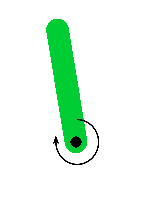
\includegraphics[width=.35\textwidth]{figs/left_leaning.pdf}
          \caption{Domain A: \\ \hspace*{0.35cm} $\alpha = 10^\circ$}
          \label{fig:left_pendulum}
        \end{subfigure}%
        \begin{subfigure}{.32\columnwidth}
            \centering
            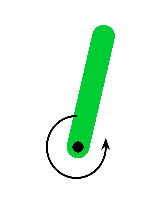
\includegraphics[width=.35\textwidth]{figs/right_leaning.pdf}
            \caption{Domain B: \\ \hspace*{0.35cm} $\alpha = -10^\circ$}
            \label{fig:right_pendulum}
        \end{subfigure}
        \begin{subfigure}{.32\columnwidth}
            \centering
            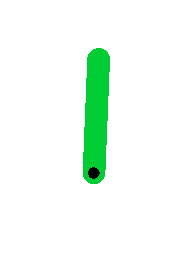
\includegraphics[width=.35\textwidth]{figs/up_leaning.pdf}
            \caption{Domain B with\\ \hspace*{0.35cm} Domain A anchor}
            \label{fig:up_pendulum}
        \end{subfigure}
        \caption{\rev{
            Policies in (a) and (b) are initially trained to lean an inverted pendulum at their respective angle $\alpha$. While in (c) the anchor-critic from the Domain A causes the resultant fine-tuned policy to hold the pendulum straight-up with no significant lean.
            Fig.\ref{fig:ddpg_anchor_pendulum} demonstrates an example of how the pendulum states evolve with time before and after adaptation.
        }}
        \label{fig:pendulum_overview}
        %\vspace{-\baselineskip}
        \end{figure}
        
        \begin{figure}[h]
            \centering
            \includegraphics[width=\columnwidth]{figs/pendulum_single_anchor_ddpg.pdf}
            \caption{
                The sin of the inverted pendulum's angle $\alpha$ over time starting from $\alpha = 90^\circ$ for a DDPG agent trained initially on Domain~A as per Fig.~\ref{fig:left_pendulum}, and then adapted to Domain~B with Domain~A anchors as per Fig.~\ref{fig:up_pendulum}.
                Note that initial training allows the agent to stably balance the pendulum to approximately $10^\circ$ while adaptation results in the agents driving the pendulum to approximately $0^\circ$.
            }
            \label{fig:ddpg_anchor_pendulum}
            \vspace{-\baselineskip}
        \end{figure}

        To test the general viability of anchor critics, we implemented them in three popular contemporary RL algorithms:~DDPG~\cite{DDPG}, SAC~\cite{SAC}, and TD3~\cite{TD3} and tested them on a modified inverted pendulum problem.
        The typical goal of the task is to stabilize a torque-controlled pendulum vertically upright, but we instead target holding the pendulum at a specified angle.
        Agents were instead trained to lean an inverted pendulum to the left while upright (Fig.~\ref{fig:left_pendulum}).
        Those agents were then retrained to lean right, but this time by using anchors from Domain A, agents were also incentivized to lean left.
        The resulting policies were observed to learn to balance the pendulum straight-up with no lean since the new rewards condition the `live' critic to motivate the policy to lean right, while the anchor critic simultaneously preserves leaning left (Fig.~\ref{fig:up_pendulum}).
        An overview of this problem is provided in Fig.~\ref{fig:pendulum_overview}.
        % Treating 0 radians as the straight upright position, we initially train an actor to point the pendulum at an angle of $\frac{\pi}{5}$ radians (meaning it should balance upright but lean to the left), and we save this actor along with its corresponding critic.
        % We then train the actor to point towards the angle $-\frac{\pi}{5}$ radians (leaning right), and we use the critic we saved earlier as an anchor. 
        % The actor is trained to point to the new set-point while preserving its performance on the anchor.
        % The resultant actor policy learns to split the difference between the current and previous goal and learns to balance the pendulum vertically upright. 
        Fig.~\ref{fig:ddpg_anchor_pendulum} demonstrates an example of this behavior for a DDPG agent.
        Additional data for more agents and for agents trained with different algorithms are available on our website \cite{supplementary} and are also discussed in the companion video for this paper.
        
        % \rev{
        % To test and demonstrate the basic efficacy of anchor critics in training, we conducted a set of simple experiments.
        % Agents were trained to lean an inverted pendulum slightly to the left while upright.
        % The agents were then fine-tuned to lean-slightly to the right with the anchor-critic conditioning agents to still lean to the left.
        % The resultant policies were observed to learn to balance the pendulum straight-up with no lean, since the new rewards condition the `live' critic to motivate the policy to lean right, while the anchor critic is simultaneously lean left.
        % These trends were observed with with multiple RL algorithmic backbones, including DDPG~\cite{DDPG}, SAC~\cite{SAC} and TD3~\cite{TD3}, additional details and data for which are provided in Appendix~\ref{A:pendulum} found on our project website: \note{ADD LINK}.
        % }

    \subsection{Testing Anchors on Gymnasium}\label{subsec:simAnchors}
        In order to evaluate the effectiveness of anchors, we perform experiments on various benchmark Gymnasium environments.
        First, we perform experiments that showcase the severity of catastrophic forgetting even when system dynamics remain the same
        We choose to divide our experiments into adaptation and 

\begin{table}[h]
\caption{Results for Pendulum-v1 and Reacher-v4 Experiments}
\label{tab:combined_results}
\centering
\begin{tabular}{c|ccc}
\hline
Parameter & Original & Naive & Anchored \\
\hline\hline
Gravity (m/s$^2$) & \multicolumn{3}{c}{Pendulum Rewards} \\
\hline
13 & 377.34$\pm$14.36 & 226.97$\pm$39.87 & 377.66$\pm$13.66 \\
4 & 352.37$\pm$69.84 & 387.47$\pm$7.48 & 370.05$\pm$53.21 \\
\hline\hline
Distance (m) & \multicolumn{3}{c}{Reacher Rewards} \\
\hline
0.1 & 330.36$\pm$39.91 & 350.96$\pm$43.90 & 336.98$\pm$46.28 \\
0.2 & 350.47$\pm$21.36 & 276.83$\pm$86.88 & 347.10$\pm$26.00 \\
\hline
\end{tabular}
\end{table}



        
        % \begin{table}[h]
        %     \caption{Errors and power consumption in flight before and after 15 steps of live adaptation}
        %     \vspace{-.5\baselineskip}
        %     \centering
        %     \begin{tabular}{c|c|c|c}
        %         \hline & {Pre-Adaptation} & {No Anchors} & {With Anchors} \\
        %         \hline
        %         Reacher & $0.8729 \pm 0.0182$ & $0.6402 \pm 0.0543$ & $0.8603 \pm 0.0319$\\
        %         Lunar Lander & $12.55 \pm 12.22$ & $14.13 \pm 5.21$ & x\\
        %         Pendulum & $12.6 \pm 0.98$ & $5.85 \pm 0.96$ & x\\
        %         \hline
        %     \end{tabular}
        %     \vspace{-1.5\baselineskip}
        % \end{table}
        % Pendulum
    % No Anchors:
% g 7  0.8282+-0.0026
% g 15 0.4361+-0.0095

% Anchored:
% g 7  0.7130+-0.0181
% g 15 0.7878+-0.0037

% Lander
% original
% wind: 53.0751+-15.7589
% no wind: 62.9119+-17.1236

% a:True
% wind: 50.3260+-11.2897
% no wind: 63.3633+-16.9065

% a:False
% wind: 26.5898+-10.5852
% no wind: 37.0747+-20.8988
    \subsection{Catastrophic Forgetting and Safety Concerns in Adaptation without Anchors}\label{subsec:forgettingAndUnsafe}
        
        Before testing adaptation in live, unconstrained flight, we first conducted a series of tests in a controlled lab environment where the drone was attached to a light tether to restrain it in the event of a catastrophic loss of control, without being a hindrance to flight.
        These tests consisted of fine-tuning a well-trained controller from simulation on the real platform while giving it typically small control targets ($< 50$ deg/s) and occasionally requesting control in excess of that ($> 100$ deg/s).
        Without anchors preserving agents' performance on larger control inputs---like those experienced during the simulated training---the live agents were observed to forget how to maintain tracking when receiving large inputs, though sometimes regaining control, and often losing it again, as seen in Fig.~\ref{fig:ac_vs_no_ac}.
        This also results in a sudden loss of control where errors would quickly snowball and motor actuation rises sharply, risking damage to the drone.
        Fig.~\ref{fig:instability} demonstrates how, when commanding attitudes not seen for a while during live-flight adaptation, agents could very quickly lose control (observed from MAEs increasing quickly and exponentially) -- which we attributed to overfitting over the relative homogeneity of the live-flight training data.
        Anchors help avoid this problem.
        
        \begin{figure}[t]
            \centering
            \includegraphics[width=\columnwidth]{figs/with_vs_without_ac.pdf}
            \caption{
                Shown here is how MAEs and smoothness evolve with adaptation steps, with and without anchors. 
                In both cases smoothness improves, however, without anchors, tracking errors often diverge wildly as catastrophic forgetting occurs and the quadrotor fails to follow larger control inputs. 
                With anchors, error is bounded and remains in controllable range.
            }
            \label{fig:ac_vs_no_ac}
            \vspace{-.5\baselineskip}
        \end{figure}
        
        \begin{figure}[t]
        \centering
        \includegraphics[width=\columnwidth]{figs/DDPGxQRegAdaptErrors.pdf}
        \caption{
            \rev{
            A snapshot of instability of the drone during an adaptation run without anchors when facing large deltas in control input.
            Observe how error increases exponentially as the drone controller enters an unrecoverable state (and eventually hitting the safety net in our tests -- as shown in this paper's companion video).
            }
        }
        \label{fig:instability}
        \vspace{-1.3\baselineskip}
    \end{figure}
        
    \subsection{Live Adaptation During Unconstrained Flight}\label{subsec:unconstrainedFlight}
    
        As a final test, we test our anchored live adaptation method in unconstrained flight outdoors (with adequate safety precautions).
        Shown in Fig.~\ref{fig:fouriers} is a comparison of control signals before and after 15 adaptation steps.
        Motor usage is reduced significantly, resulting in improved control smoothness and almost a 50\% reduction in power consumption, with comparable MAEs to agents trained in simulation.
        This is further demonstrated in Table~\ref{tab:error_amps}, which examines how MAE, smoothness, and current draw change through adaptation.

        \begin{table}[h]
            \caption{Errors and power consumption in flight before and after 15 steps of live adaptation}
            \vspace{-.5\baselineskip}
            \label{tab:error_amps}
            \centering
            \begin{tabular}{c|c|c}
                \hline & {Before Adaptation} & {After Adaptation} \\
                \hline
                Amperage $\downarrow$ & $13.7 \pm 8.47$ & $7.24 \pm 3.97$\\
                Mean Average Error $\downarrow$ & $12.55 \pm 12.22$ & $14.13 \pm 5.21$\\
                Smoothness $\times 10^{4}$ $\downarrow$ & $12.6 \pm 0.98$ & $5.85 \pm 0.96$ \\
                \hline
            \end{tabular}
            \vspace{-1.5\baselineskip}
        \end{table}
        
        \begin{figure}[h]
            \centering
            \includegraphics[width=\columnwidth]{figs/before_after_adapt.pdf}
            \caption{
                Comparisons of motor usage during flight and corresponding FFTs demonstrate the improvement in smoothness after adaptation, as noted from the reduction in high-frequency components on the FFT amplitude plot. 
                While the motor usage plot samples a single trajectory for clarity, the FFTs are averaged over multiple adaptations to demonstrate repeatability.
            }
            \label{fig:fouriers}
            \vspace{-1.5\baselineskip}
        \end{figure}
        

        
    \subsection{A Case Against Mixing Replay Buffers During Adaptation}\label{subsec:mixedBuffers}
        
        It may seem reasonable, as a first-pass solution, to fine-tune agents for real flight by mixing simulated and real data during fine-tuning.
        However, theoretically, training a single critic with a mixture of data from two separate environments would violate the RL algorithms’ Markovian assumption.
        The different environments have different dynamics so their implicit transition functions would depend on a now hidden state not represented in our state space, namely which environment it comes from.
        One could possibly include this, however this would necessitate a change in the agents' input structure and corresponding controller NN model architecture.
        We therefore instead opted to maintain two separate Q-value functions and replay buffers. 
        Separating the Q-value functions also enables weighing how much actors ‘care’ about optimizing one value function over the other, allowing us to tune how much we trade off stability over adaptability and vice versa.

    \subsection{Known Limitations}\label{subsec:limitations}

        Both \framework{} and the anchored learning techniques discussed in this work demonstrate a clear utility in sim-to-real control transfer and live adaptation of learned controllers on a compute-constrained platform.
        However, even with the improvements we demonstrate, we are not yet able to surpass the performance of the PPO algorithm on TF1 with any of the algorithms tested so far on TF2.
        Furthermore, while anchors clearly help improve control smoothness without resulting in catastrophic forgetting, the adapted agents were not observed to improve their tracking performance, even though this remained the key learning objective of the policy optimization.
        It is as yet unclear as to whether this is simply a limitation of the DDPG algorithm (or our specific implementation), or a matter of how the regularization was tuned.
        Finally, even though we demonstrate that anchors can be helpful in preserving behaviors from one environment when fine-tuning an agent on another, the optimization structure forces a performance compromise.
        While this helps prevent forgetting, it also prevents policies from adopting substantially new and potentially more effective behaviors.
        This is by design, of course, but in cases where domain gaps are large, the very stability offered by the anchor critics may significantly compromise fine-tuning of behavior and could result in policies that are ill-suited for both the initial and transferred domain. 
        Another limitation is our use of a saved replay buffer from simulation to evaluate anchor critics. While this worked in our experiments, we suspect that keeping the simulation in the loop might allow for anchors to better represent simulation performance.

    

%%%%%%%%%%%%%%%%%%%%%%%%%%%%%%%%%%%%%%%%%%%%%%%%%%%%%%%%%%%%%%%%%%%%%%%%%%%%%%%%
\section{BACKGROUND}

    \firmware{} is an evolution of Neuroflight, initially developed by Koch~et~al.~\cite{NFori, NFv2}.
    Neuroflight extends the open-source Betaflight~\cite{betaflight-homepage} flight-control firmware stack allowing NN models to be compiled and embedded into the control firmware.
    This capability enables NN-based flight control.
    Many problems afflicted the original Neuroflight stack, most prominently, (i) high variance in training and (ii) poor sim-to-real transfer of trained agents (iii) lack of flexibility in swapping NN controllers live.
    In many cases, trained controllers exhibited worse control and high power consumption than would be expected from their simulated performance. 
    Some of these issues were addressed in follow-up works mainly via a multiplicative reward shaping technique (RE+AL)~\cite{mysore2021train} and via regularizing policies for incentivizing smoothness in control outputs~\cite{mysore2021caps} (CAPS).
    Importantly, these works enabled significant savings in power consumption, outperforming even fully-tuned PID controllers and filters, even though they were only trained in simulation.
    However, the performance of such policies is inherently limited by the differences between the simulation's dynamics and the dynamics of reality (known as the sim-to-real gap).
    Limitations in the design of the Neuroflight tool-chain force NN controllers to be statically embedded into the robot's firmware, precluding the ability to perform controller adaptation.
    
\section{RELATED WORK}   
    \begin{itemize}
        \item Liquid neural nets
        \item hebbian plasticity
    \end{itemize}
    Work exploring controller-based live-adaptivity can be divided into either model-based or model-free approaches. 
    In classical control theory~\cite{PasikDuncan1996AdaptiveC}, given a family of models, adaptation is defined as being synonymous with identifying the parameters for the optimal model from observations. 
    Techniques based on this theory have been used for quadrotor control as well~\cite{model_quad_adapt}. 
    % More recently, advances were made for adaptation on more challenging control problems by employing model based reinforcement learning \cite{Song2020ProvablyEM}. 
    More recent advances have sought to tackle adaptation in more challenging control problems by employing model-based reinforcement learning~\cite{Song2020ProvablyEM}. 
    Model-based RL techniques are, however, constrained by difficulties in accurately modeling the dynamics of real systems.
    Meta RL has also been proposed as a model-free solution for adaptivity, where policies are trained to adapt to different environments~\cite{MetaSimToReal, Nagabandi2019LearningTA, Dextrous}. 
    However, these techniques rely on being able to identify and vary simulator parameters to maximally cover a wide array of possible distributional shifts in order to enable policies to adapt to real-life scenarios. 
    They are therefore limited by how much simulated environments can represent unexpected shifts in the dynamics of reality. 
    Other methods directly employ RL, either via on-board compute, or via immediate communication, however, safety is often a concern under arbitrary policies. 
    Cheng~et~al.~\cite{Cheng_Orosz_Murray_Burdick_2019} attempt to address this by allowing only safe exploration, but again rely on being able to model safety criteria. 
    Other methods focus on keeping policies within a `trust region' during optimization, to improve stability and prevent large changes in behavior~\cite{TRPO,PPO}. This approach is similar to ours in that it tries to preserve existing behavior, but anchor critics instead incentivizes finding policies that perform well both in simulation and reality, rather than constrain the policy to not change in behavior. These ideas end up being orthogonal, as both can be applied.

    
%%%%%%%%%%%%%%%%%%%%%%%%%%%%%%%%%%%%%%%%%%%%%%%%%%%%%%%%%%%%%%%%%%%%%%%%%%%%%%%%

\section{CONCLUSION}\label{sec:conclusion}
    
    Our work introduced the \firmwarelong{} System (\framework{}), a framework for enabling live adaptation of neural network based flight control for drones, or indeed any other Betaflight compatible platform.
    Our full-stack software enables ground-to-drone communication so that agents' observations during flight can be transmitted back to a ground-station for controller adaptation, with the adapted controllers being transferred back to the drone, which the drone can seamlessly swap to without compromising the control loop.
    We also introduce a novel framing of the RL optimization criteria, and introduce anchor critics as a tool to stabilize sim-to-real adaptation.
    As we demonstrate, the introduction of anchor critics can significantly improve behavior retention while still giving policies enough slack to adapt themselves to new data.
    This was shown to substantially improve control smoothness and reduce power consumption without degradation in control input tracking performance.

%%%%%%%%%%%%%%%%%%%%%%%%%%%%%%%%%%%%%%%%%%%%%%%%%%%%%%%%%%%%%%%%%%%%%%%%%%%%%%%%

% \section{MATH}

% Before you begin to format your paper, first write and save the content as a separate text file. Keep your text and graphic files separate until after the text has been formatted and styled. Do not use hard tabs, and limit use of hard returns to only one return at the end of a paragraph. Do not add any kind of pagination anywhere in the paper. Do not number text heads-the template will do that for you.

% Finally, complete content and organizational editing before formatting. Please take note of the following items when proofreading spelling and grammar:

% \subsection{Abbreviations and Acronyms} Define abbreviations and acronyms the first time they are used in the text, even after they have been defined in the abstract. Abbreviations such as IEEE, SI, MKS, CGS, sc, dc, and rms do not have to be defined. Do not use abbreviations in the title or heads unless they are unavoidable.

% \subsection{Units}

% \begin{itemize}

% \item Use either SI (MKS) or CGS as primary units. (SI units are encouraged.) English units may be used as secondary units (in parentheses). An exception would be the use of English units as identifiers in trade, such as Ò3.5-inch disk driveÓ.
% \item Avoid combining SI and CGS units, such as current in amperes and magnetic field in oersteds. This often leads to confusion because equations do not balance dimensionally. If you must use mixed units, clearly state the units for each quantity that you use in an equation.
% \item Do not mix complete spellings and abbreviations of units: ÒWb/m2Ó or Òwebers per square meterÓ, not Òwebers/m2Ó.  Spell out units when they appear in text: Ò. . . a few henriesÓ, not Ò. . . a few HÓ.
% \item Use a zero before decimal points: Ò0.25Ó, not Ò.25Ó. Use Òcm3Ó, not ÒccÓ. (bullet list)

% \end{itemize}


% \subsection{Equations}

% The equations are an exception to the prescribed specifications of this template. You will need to determine whether or not your equation should be typed using either the Times New Roman or the Symbol font (please no other font). To create multileveled equations, it may be necessary to treat the equation as a graphic and insert it into the text after your paper is styled. Number equations consecutively. Equation numbers, within parentheses, are to position flush right, as in (1), using a right tab stop. To make your equations more compact, you may use the solidus ( / ), the exp function, or appropriate exponents. Italicize Roman symbols for quantities and variables, but not Greek symbols. Use a long dash rather than a hyphen for a minus sign. Punctuate equations with commas or periods when they are part of a sentence, as in

% $$
% \alpha + \beta = \chi \eqno{(1)}
% $$

% Note that the equation is centered using a center tab stop. Be sure that the symbols in your equation have been defined before or immediately following the equation. Use Ò(1)Ó, not ÒEq. (1)Ó or Òequation (1)Ó, except at the beginning of a sentence: ÒEquation (1) is . . .Ó

% \subsection{Some Common Mistakes}
% \begin{itemize}


% \item The word ÒdataÓ is plural, not singular.
% \item The subscript for the permeability of vacuum ?0, and other common scientific constants, is zero with subscript formatting, not a lowercase letter ÒoÓ.
% \item In American English, commas, semi-/colons, periods, question and exclamation marks are located within quotation marks only when a complete thought or name is cited, such as a title or full quotation. When quotation marks are used, instead of a bold or italic typeface, to highlight a word or phrase, punctuation should appear outside of the quotation marks. A parenthetical phrase or statement at the end of a sentence is punctuated outside of the closing parenthesis (like this). (A parenthetical sentence is punctuated within the parentheses.)
% \item A graph within a graph is an ÒinsetÓ, not an ÒinsertÓ. The word alternatively is preferred to the word ÒalternatelyÓ (unless you really mean something that alternates).
% \item Do not use the word ÒessentiallyÓ to mean ÒapproximatelyÓ or ÒeffectivelyÓ.
% \item In your paper title, if the words Òthat usesÓ can accurately replace the word ÒusingÓ, capitalize the ÒuÓ; if not, keep using lower-cased.
% \item Be aware of the different meanings of the homophones ÒaffectÓ and ÒeffectÓ, ÒcomplementÓ and ÒcomplimentÓ, ÒdiscreetÓ and ÒdiscreteÓ, ÒprincipalÓ and ÒprincipleÓ.
% \item Do not confuse ÒimplyÓ and ÒinferÓ.
% \item The prefix ÒnonÓ is not a word; it should be joined to the word it modifies, usually without a hyphen.
% \item There is no period after the ÒetÓ in the Latin abbreviation Òet al.Ó.
% \item The abbreviation Òi.e.Ó means Òthat isÓ, and the abbreviation Òe.g.Ó means Òfor exampleÓ.

% \end{itemize}


% \section{USING THE TEMPLATE}

% Use this sample document as your LaTeX source file to create your document. Save this file as {\bf root.tex}. You have to make sure to use the cls file that came with this distribution. If you use a different style file, you cannot expect to get required margins. Note also that when you are creating your out PDF file, the source file is only part of the equation. {\it Your \TeX\ $\rightarrow$ PDF filter determines the output file size. Even if you make all the specifications to output a letter file in the source - if your filter is set to produce A4, you will only get A4 output. }

% It is impossible to account for all possible situation, one would encounter using \TeX. If you are using multiple \TeX\ files you must make sure that the ``MAIN`` source file is called root.tex - this is particularly important if your conference is using PaperPlaza's built in \TeX\ to PDF conversion tool.

% \subsection{Headings, etc}

% Text heads organize the topics on a relational, hierarchical basis. For example, the paper title is the primary text head because all subsequent material relates and elaborates on this one topic. If there are two or more sub-topics, the next level head (uppercase Roman numerals) should be used and, conversely, if there are not at least two sub-topics, then no subheads should be introduced. Styles named ÒHeading 1Ó, ÒHeading 2Ó, ÒHeading 3Ó, and ÒHeading 4Ó are prescribed.

% \subsection{Figures and Tables}

% Positioning Figures and Tables: Place figures and tables at the top and bottom of columns. Avoid placing them in the middle of columns. Large figures and tables may span across both columns. Figure captions should be below the figures; table heads should appear above the tables. Insert figures and tables after they are cited in the text. Use the abbreviation ÒFig. 1Ó, even at the beginning of a sentence.

% \begin{table}[h]
% \caption{An Example of a Table}
% \label{table_example}
% \begin{center}
% \begin{tabular}{|c||c|}
% \hline
% One & Two\\
% \hline
% Three & Four\\
% \hline
% \end{tabular}
% \end{center}
% \end{table}


%   \begin{figure}[thpb]
%       \centering
%       \framebox{\parbox{3in}{We suggest that you use a text box to insert a graphic (which is ideally a 300 dpi TIFF or EPS file, with all fonts embedded) because, in an document, this method is somewhat more stable than directly inserting a picture.
% }}
%       %\includegraphics[scale=1.0]{figurefile}
%       \caption{Inductance of oscillation winding on amorphous
%       magnetic core versus DC bias magnetic field}
%       \label{figurelabel}
%   \end{figure}
   

% Figure Labels: Use 8 point Times New Roman for Figure labels. Use words rather than symbols or abbreviations when writing Figure axis labels to avoid confusing the reader. As an example, write the quantity ÒMagnetizationÓ, or ÒMagnetization, MÓ, not just ÒMÓ. If including units in the label, present them within parentheses. Do not label axes only with units. In the example, write ÒMagnetization (A/m)Ó or ÒMagnetization {A[m(1)]}Ó, not just ÒA/mÓ. Do not label axes with a ratio of quantities and units. For example, write ÒTemperature (K)Ó, not ÒTemperature/K.Ó

% \section{CONCLUSIONS}

% A conclusion section is not required. Although a conclusion may review the main points of the paper, do not replicate the abstract as the conclusion. A conclusion might elaborate on the importance of the work or suggest applications and extensions. 

% \addtolength{\textheight}{-12cm}   % This command serves to balance the column lengths
%                                   % on the last page of the document manually. It shortens
%                                   % the textheight of the last page by a suitable amount.
%                                   % This command does not take effect until the next page
%                                   % so it should come on the page before the last. Make
%                                   % sure that you do not shorten the textheight too much.

%%%%%%%%%%%%%%%%%%%%%%%%%%%%%%%%%%%%%%%%%%%%%%%%%%%%%%%%%%%%%%%%%%%%%%%%%%%%%%%%


%%%%%%%%%%%%%%%%%%%%%%%%%%%%%%%%%%%%%%%%%%%%%%%%%%%%%%%%%%%%%%%%%%%%%%%%%%%%%%%%

\bibliographystyle{IEEEtran}
\bibliography{references.bib}
\clearpage
\newpage
%%%%%%%%%%%%%%%%%%%%%%%%%%%%%%%%%%%%%%%%%%%%%%%%%%%%%%%%%%%%%%%%%%%%%%%%%%%%%%%%
\appendix

\subsection{\rev{\firmware{} System Transceiving Metrics}}\label{A:comms_metrics}
        \rev{
        Using the Transceiving framework and hardware described in Section~\ref{sec:firmware}, i.e MATEK-F722 controller equipped with ZigBee\textsuperscript{\circledR}-PRO  radio-frequency modules, transmission and switching time for NNs were measured.
        The control networks used in this work use two hidden layers with 32 neurons each.
        We employ a transmission baudrate of 115200 to send NNs of 8mb, which takes 11~s to transfer between the ground station and the drone -- receiving is handled in parallel to the flight control, so the drone is able to remain fully operational while waiting for a new network.
        When a network is received, switching to the new NN controller takes 134 ms.
        During flight, the drone also transmits state observations of 59 bytes back to the ground station, transmitting 244 observations per second.
        }
        
    \begin{figure*}[t]
        \centering
        \begin{subfigure}[h]{0.32\textwidth}
            \centering
            \includegraphics[width=\textwidth]{figs/pendulum_anchor_ddpg.pdf}
            \caption{DDPG}
            \label{fig:pendulum_ddpg}
        \end{subfigure}
        \begin{subfigure}[h]{0.32\textwidth}
            \centering
            \includegraphics[width=\textwidth]{figs/pendulum_anchor_sac.pdf}
            \caption{SAC}
            \label{fig:pendulum_sac}
        \end{subfigure}
        \begin{subfigure}[h]{0.32\textwidth}
            \centering
            \includegraphics[width=\textwidth]{figs/pendulum_anchor_td3.pdf}
            \caption{TD3}
            \label{fig:pendulum_td3}
        \end{subfigure}
        \caption{\rev{Evolution of the angle ($sin(\theta)$) of an inverted pendulum over time for policies trained with anchor-critics tested on DDPG, SAC and TD3.
        There are 5 different test runs per goal, and the angle of the pendulum is initialized at random.
        All 3 anchored algorithms consistently learn to point to 0 rad, thus maintaining a good compromise between our initial goal and our new goal.}}
        \label{fig:pendulum_all}
    \end{figure*}    
    
% \subsection{\rev{Anchor-Critics: Inverted Pendulum Test}}\label{A:pendulum}
    
%     % \rev{
%     % To test the general viability of anchor critics, we implemented them in three popular contemporary RL algorithms: DDPG, SAC, and TD3.
%     % We tested the anchors on a modified inverted pendulum problem.
%     % The typical goal of the task is to stabilize a torque-controlled pendulum vertically upright, but we modified it to instead target holding the pendulum at a specified angle.
%     % Treating 0 radians as the straight upright position, we initially train an actor to point the pendulum at an angle of $\frac{\pi}{5}$ radians (meaning it should balance upright but lean to the left), and we save this actor along with its corresponding critic.
%     % We then train the actor to point towards the angle $-\frac{\pi}{5}$ radians (leaning right), and we use the critic we saved earlier as an anchor. 
%     % The actor is trained to point to the new set-point but while preserving its performance on the anchor.
%     % The resultant actor policy learns to split the difference between the current and previous goal and learns to balance the pendulum vertically upright, as shown in Fig.~\ref{fig:pendulum_all}.
%     % }

    % \begin{figure}[t]
    %     \centering
    %     \includegraphics[width=\columnwidth]{figs/DDPGxQRegAdaptErrors.pdf}
    %     \caption{
    %         \rev{
    %         A snapshot of instability of the drone during an adaptation run without anchors when varying the control input.
    %         Due to a lot of the real-world training data mostly comprising of smaller movements, the agents over-fit to this and forget to handle more aerobatic maneuvers learned in simulation.
    %         Observe how error increases exponentially as the drone controller enters an unrecoverable state. 
    %         In our tests, the inclusion of the anchor was found to mitigate this issue by preventing catastrophic forgetting and ensuring that agents continue to `care' about simulated training maneuvers.
    %         }
    %     }
    %     \label{fig:instability}
    %     \vspace{-1.5\baselineskip}
    % \end{figure}

\subsection{\rev{Hyper-parameter search}}\label{A:hypersearch}
    \rev{
    We conducted a hyper-parameter search and a correlation factor analysis using 4 different prominent RL algorithms -- PPO, DDPG, SAC and TD3 -- for the quadrotor attitude control problem mainly considered in this paper. 
    The list of tested hyper-parameters and their corresponding correlations to the training reward are presented in Tables~\ref{tab:ppo_corr},~\ref{tab:ddpg_corr},~\ref{tab:sac_corr}~and~\ref{tab:td3_corr} respectively.
    Our hyper-parameter choices were informed by common values used to achieve the best performance across various benchmark Gymnasium environments~\cite{rl-zoo}.
    }
    
    \rev{
    Table~\ref{tab:alg_comp} meanwhile compares the training performances of each of the algorithms, as well as DDPG$\times$ which we introduce in this work, after 300000 training steps (corresponding to a quarter of our typical training time and the time by which DDPG$\times$ typically starts to plateau), but on a slightly modified version of the problem -- where agents are only required to minimize tracking error, without worrying about other characteristics such as control smoothness.
    This, we found, was typically a good starting point for tuning algorithms' hyper-parameters and to determine if they are capable of addressing the underlying control problem.
    As the data demonstrates, all the tested algorithms perform significantly worse than DDPG$\times$.
    }
    
    \rev{
    While the relative performance metrics appear similar across DDPG, PPO, SAC and TD3, there are critical differences in the quality of the behaviors being learned, which in turn impacts the ability of the algorithms to further improve agents' performances.
    As shown in Fig.~\ref{fig:ppovppo2vddpgx}, the tested TF2 implementation of PPO does not behave similarly to the modified OpenAI Baselines~\cite{baselines} TF1 version used in previous work.~\cite{mysore2021caps,mysore2021train, NFv2}.
    Where the PPO based on Baselines learns to track the control signals well, albeit with high variance in the motor actuation (since smoothness is not being trained for), the TF2 implementation saturates the motor commands at the maximum, thus effectively doing nothing to control the drone's attitude.
    This still generates some reward, since the training environment predominantly consists of smaller (but more frequently varying) control angular velocities.
    The problem with this, however, is that this behavior seems to be a local optima that is difficult for the algorithms to recover from to further improve performance.
    }
    
    \rev{
    When considering alternatives to PPO, we experimented with Q-learning-based DDPG, SAC and TD3.
    As shown in Fig.~\ref{fig:ddpgvsacvtd3}, we observed that TD3 would often fall into similar trappings as PPO, with the motor outputs becoming saturated at maximum actuation.
    While DDPG was slower to learn (often performing worse than SAC), crucially, it did not saturate and would in fact consistently try to maintain control through more nuanced use of the motors -- an extreme but illustrative case is shown in Fig.~\ref{fig:ddpgvsacvtd3}.
    Given our results, while SAC would have been preferable as a starting point based on the typical rewards achieved, the fact remained that training SAC was approximately 1.5 times slower than DDPG for relatively marginal gains, making it a less attractive option for iterating.
    DDPG was therefore deemed the best contender with which to experiment on our proposed multiplicative policy optimization.
    In our tests, agents which achieve an average reward of more 0.8 were typically responsive enough to control in real flight.
    }
    
    \begin{table*}[t]
        \centering
        \caption{\rev{This table shows the performance of the different RL algorithms over the aforementioned environment. Training ends after invoking the environment 300,000 times and is tested 5 times for every hyperparameter sample.
        The reward value is then computed for every sample of hyperparameters of which there are at least 10 samples per algorithm. 
        Step times are reported for a desktop running Ubuntu v 18.04 with an Intel Core i7-7700 CPU (no GPU optimization is used since training is primarily CPU limited).} 
        }
        \vspace{.5\baselineskip}
        \rev{
        \begin{tabular}{c|c|c|c|c|c}
            \hline
            Algorithm & DDPG$\times$ & DDPG & PPO (TF2) & SAC & TD3 \\ \hline
            Reward  & $0.89\pm0.033$ & $0.38\pm0.13$ & $0.36\pm0.11$ & $0.40\pm0.12$ & $0.37\pm0.11$ \\
            Max Reward & 0.93 & 0.59 & 0.61 & 0.63 & 0.57 \\
            Step time (s) & $9.6 \times 10^{-3}$ & $9.6 \times 10^{-3}$ & $3.6 \times 10^{-3}$ & $1.44 \times 10^{-2}$ & $1.2 \times 10^{-2}$ \\ \hline
        \end{tabular}
        }
        \label{tab:alg_comp}
    \end{table*}
    
    \begin{table*}[t]
        \centering
        \caption{\rev{TF2 PPO paramater/reward correlations}}
        \rev{
        \begin{tabular}{c|c|c}
            \hline
            Parameter   & Correlation & Tested Values \\ \hline
            Clip ratio  &  0.098 & [0.0, 0.05, 0.1, 0.2] \\ 
            $\gamma$       & -0.100 & [0.8, 0.9, 0.95, 0.99]\\ 
            Policy learning rate       &  0.679 & [1e-4, 5e-4, 1e-3, 3e-3, 5e-3] \\ 
            Value learning rate       &  0.255 & [1e-4, 5e-4, 1e-3, 3e-3, 5e-3] \\
            lam         &  0.056 & [0.9, 0.97, 0.99, 0.995] \\ \hline
        \end{tabular}
        }
        \label{tab:ppo_corr}
    \end{table*}
    
    \begin{table*}[t]
        \centering
        \caption{\rev{DDPG paramater/reward correlations}}
        \rev{
        \begin{tabular}{c|c|c}
            \hline
            Parameter   & Correlation & Tested Values \\ \hline
            Replay buffer size  & -0.156 & [100 000, 500 000, 1000 000, 5000 000] \\
            $\gamma$        & -0.161 & [0.8, 0.9, 0.95, 0.99] \\
            Polyak       &  0.203 & [0.5, 0.9, 0.95, 0.99, 0.995] \\
            Policy learning rate        & -0.211 & [1e-4, 5e-4, 1e-3, 3e-3, 5e-3] \\
            Critic learning rate         & -0.676 & [1e-4, 5e-4, 1e-3, 3e-3, 5e-3] \\
            Batch size   & -0.142 & [50, 100, 200, 400] \\
            Action noise    & -0.691 & [0.01, 0.05, 0.1, 0.2] \\ \hline
        \end{tabular}
        }
        \label{tab:ddpg_corr}
    \end{table*}
    
    
    \begin{table*}[t]
        \centering
        \caption{\rev{SAC paramater/reward correlations}}
        \rev{
        \begin{tabular}{c|c|c}
            \hline
            Parameter    & Correlation & Tested Values \\ \hline
            Replay buffer size  & -0.088 & [100 000, 500 000, 1000 000, 5000 000] \\
            $\gamma$        &  0.272 & [0.8, 0.9, 0.95, 0.99] \\
            Polyak       &  0.102 & [0.5, 0.9, 0.95, 0.99, 0.995] \\
            Learning Rate           & -0.256 & [1e-4, 5e-4, 1e-3, 3e-3, 5e-3] \\
            $\alpha$        &  0.356 & [0.01, 0.05, 0.1, 0.2] \\
            Batch size   &  0.866 & [50, 100, 200, 400] \\ \hline
        \end{tabular}
        }
        \label{tab:sac_corr}
    \end{table*}
    
    \begin{table*}[t]
        \centering
        \caption{\rev{TD3 paramater/reward correlations}}
        \rev{
        \begin{tabular}{c|c|c}
            \hline
            Parameter    & Correlation & Tested Values \\ \hline
            Replay buffer size  &  0.516 & [100 000, 500 000, 1000 000, 5000 000] \\
            $\gamma$        &  0.479 & [0.8, 0.9, 0.95, 0.99] \\
            Polyak       &  0.007 & [0.5, 0.9, 0.95, 0.99, 0.995] \\
            Policy learning rate        & -0.430 & [1e-4, 5e-4, 1e-3, 3e-3, 5e-3] \\
            Critic learning rate         &  0.023 & [1e-4, 5e-4, 1e-3, 3e-3, 5e-3] \\
            Batch size   &  0.118 & [50, 100, 200, 400] \\
            Act noise    &  0.313 & [0.01, 0.05, 0.1, 0.2] \\ \hline
        \end{tabular}
        }
        \label{tab:td3_corr}
    \end{table*}
    
    \begin{figure}[t]
        \centering
        \includegraphics[width=\columnwidth]{figs/PPOvPPO2vDDPGx.pdf}
        \caption{
            \rev{
            A snapshot of PPO and DDPG$\times$ agents after 300,000 training steps acting in their training environment.
            Attitude control elements are split into Yaw, Pitch, and Roll in the left column.
            On the right are the outputs generated by the agents while attempting to follow the control inputs.
            Without smoothness considerations, within 300,000 steps, Baselines PPO performs very well on tracking while outputting actions with high variability (as is shown in previous works \cite{mysore2021caps}, \cite{mysore2021train}).
            Conversely, the TF2 implementation of PPO fails to learn useful behavior across hyper-parameters.
            DDPG$\times$, which we introduced in this work, is able to reasonably follow the target while maintaining smooth outputs and continues to improve as training progresses.
            }
        }
        \label{fig:ppovppo2vddpgx}
        \vspace{-1.5\baselineskip}
    \end{figure}
    
    
    
    \begin{figure}[t]
        \centering
        \includegraphics[width=\columnwidth]{figs/DDPGvSACvTD3.pdf}
        \caption{
            \rev{
                For the three DDPG-based algorithms, we observe clear dissimilarities in the quality of the policies learned, based on input tracking and motor usage.
                Entropy regularization employed in SAC allows trained agents to achieve relatively reasonable performance on both tracking and motor usage, but the algorithm was noted to not improve further with more training, likely due to the same regularization that initially helps preventing large responses, thus preventing the algorithm from learning to track more aggressive maneuvers.
                TD3 behaves similarly to the TF2 PPO, in that it tends to saturate at various local optima, outputting extreme values.
                DDPG, on the other hand, demonstrates some tracking capabilities can varies its control output drastically when close to the setpoint, similar in behavior to Baselines PPO. 
                Given these three candidate algorithms and their relative benefits and drawbacks, we chose to modify DDPG as it runs faster than SAC and was capable of achieving good tracking performance.
                While DDPG itself was not consistently reliable, DDPG$\times$, with our proposed improvements, was repeatable and controllable.
            }
        }
        \label{fig:ddpgvsacvtd3}
        \vspace{-1.5\baselineskip}
    \end{figure}

    %%%%%%%%%%%%%%%%%%%%%%%%%%%%%%%%%%%%%%%%%%%%%%%%%%%%%%%%%%%%%%%%%%%%%%%%%%%%%%%%
\section{TRAINING FLIGHT CONTROLLERS WITH \framework{}}

    Prior work employing the Neuroflight training framework trained RL-based controllers using TF1~\cite{NFori, NFv2, mysore2021train, mysore2021caps}.
    Attempting to deploy these RL-based controllers using our updated stack with TFLite's interpreter resulted in the control firmware crashing during invocation,
    \rev{due to the operations used by the translated TFv1 NNs.}
    % Without a development version of the MATEK-F722 controller, 
    % or an accessible JTAG, we were, unfortunately, unable to debug the source(s) of these issues.
    % Agents built with TensorFlow-v2, within the constraints of the operations supported by TFLite, could be successfully deployed and invoked.
    Agents built with TF2, conversely, could be successfully deployed and invoked.
    This compelled us to update our training stack to TF2.
    
    Transitioning to TF2 introduced a problem for the training pipeline.
    Prior works \cite{mysore2021caps, mysore2021train, NFv2} train flight-control agents with the OpenAI Baselines~\cite{baselines} implementation of PPO~\cite{PPO}.
    While reproducible with the software packages and versions reported by the authors, the performance observed with PPO agents in TF1 was not achievable by any of several tested TF2 implementations of PPO, including TF-agents~\cite{TFAgents}, stable-baselines~\cite{stable-baselines} etc., despite using identical network architectures and performing a full hyperparameter search.
    % This was not entirely surprising, as algorithms such as PPO and TRPO~\cite{TRPO} are known to be sensitive to (and even brittle under) implementation specifics~\cite{henderson2018deep, islam2017reproducibility, Engstrom2020Implementation}.
    Algorithms like PPO and TRPO~\cite{TRPO} are known to be sensitive to (and even brittle under) implementation specifics~\cite{henderson2018deep, islam2017reproducibility, Engstrom2020Implementation}, prompting a search for alternatives.
    
    Viable flight-control policies were trainable using a TF2 translation of OpenAI's Spinning Up~\cite{SpinningUp2018} PyTorch implementation of DDPG~\cite{DDPG}.
    While vanilla DDPG presented with similar oscillatory behavior identified in the work on CAPS ~\cite{mysore2021caps}, introducing CAPS regularization to DDPG enabled the training of viable agents in simulation.
    We found, however, that the performance of DDPG on the control problem at hand exhibited relatively high variance: not all the trained agents were safely flyable. This prompted us to explore alternative formulations which improve upon CAPS defined in the next section.
%%%%%%%%%%%%%%%%%%%%%%%%%%%%%%%%%%%%%%%%%%%%%%%%%%%%%%%%%%%%%%%%%%%%%%%%%%%%%%%%


\end{document}
